
%%%%%%%%%%%%%%%%%%%%%%%%%%%%%%%%%%%%%%%%%%%%%%%%%%%%%%%%%%%%%%%%%%%%%%%%%%%%
% This will help you in writing your report
% Remember that the character % is a comment in latex

% Divide the work you have done in each of the esers 
% in a new chapter, as in the example below, 
% using a coherent title 


% Follows some examples to include HDL, figures, ... :

%-----------------------------
% VHDL file, using the sintax:


	%\begin{listato}
	%\lstinputlisting{./exeMPLE/listato1.vhd}
	%\end{listato}

% the path to the file must be correct, obviously
% Should you have listings written in other languages the method is the 
% same one, but the language set up must be changed using a different 
% setting for the command \lstset{language=VHDL} in file homebook.tex 


%-----------------------------
% figures in postcript (ps) or encapsulated postcript (eps)
% format, using the syntax:

%	\begin{figure}[h]
%	\centering
%	\includegraphics[width=9cm]{./cap1/figure1.eps}
%	\caption{Put a caption if you want (didascalia...:)))}
%	\eserel{put-a-eserel-for-referring-to-this-picture}	
%	\end{figure}

% the path to the file must be correct, obviously
% you can refer to this picture in any point of your document
% by typing the instruction:

% 	\ref{put-a-eserel-for-referring-to-this-picture}

% that is using the same eserel you put in the fiure eserel
% when you will run the "latex command" an automatic reference to
% this figure with the correct enumeration will be inserted


%-----------------------
% comment in text format (if you are not skilled in latex and don't want to be)
% using the sintax:

	%\begin{verbatim}
	% besereserla 
	%\end{verbatim}

% The verbatimg includes text as it is, as you could write in a normal text file 

% (BETTER) If uou want to write enhancing all the latex possibilities you 
% should add to you text a few commands in some particular cases. 
% In the following you have and example of a few chapters roughtly commented
% and written all in this file: remember that you can saparate
% each chapter in different files (this is always what a latex pro does) 
% and include them using the instruction: \input{./directoryxx/fileyy.tex}


%%%%%%%%%%%%%%%%%%%%%%%%%%%%%%%%%%%%%%%%%%%%%%%%%%%%%%%%%%%%%%%%%%%%%%%%%%%%%%%
%%%%%%%%%%%%%%%%%%%%%%%%%%%%%%%%%%%%%%%%%%%%%%%%%%%%%%%%%%%%%%%%%%%%%%%%%%%%%%%%%
%%%%%%%%%%%%%%%%%%%%%%%%%%%%%%
% Beginning of Document content

% eser 1
\section{Exercise 1: Assembly of the PDN netlist}

%%%%%%%%%%%%%%%%%%%%%%%%%%%%%%%%%%%%%%%%%%%%%%%%%%%%%%%%%%%

\subsection{Analysis of the provided models}

The PDN under analysis is described by three modules: the board, the package and the die. Before connecting them, the structure of each module has
been analysed, with particular attention to its ports, since these determine how the modules can be interconnected.

\begin{itemize}
    \item \textbf{Board}: The file \texttt{board\_passive.cir} contains the subcircuit \texttt{board\_passive}, a passive SPICE macromodel generated
    automatically by IdEM from the S-parameters of the board (\texttt{board.ts}) through a rational fitting over a 5~GHz bandwidth.\\ The model has two
    ports: port~1 is connected to the VRM, and port~2 to the package (VDD balls grouped together and GND balls grouped together). The model also
    accounts for the decoupling capacitors embedded in the board, for the parasitics of the VRM and for the other passive components of the board.
    \item \textbf{Package}: The file \texttt{package\_ports\_on\_caps\_passive.cir} contains the subcircuit\\
    \texttt{package\_ports\_on\_caps\_passive}, a macromodel of the same type obtained from the\\ S-parameters of the four-layer package
    (\texttt{package\_ports\_on\_caps.ts}).\\ It has seven ports: five ports placed on the locations of the decoupling capacitors
    (\texttt{VDD\_C01\_1}, \dots, \texttt{VDD\_C05\_1}), one port on the board side (the balls, with VDD and GND grouped) and one port on the die
    side (the bumps, with VDD and GND grouped). The ports on the capacitor locations make it possible to connect the decoupling capacitors externally,
    without modifying the package model.
    \item \textbf{Die}: The file \texttt{die\_model.sp} contains the subcircuit \texttt{die\_model}, which has two terminals, \texttt{vdd} and
    \texttt{vss}. Between them there are a current source, defined as a piecewise-linear (PWL) waveform, and an equivalent RC network
    (\texttt{passive\_network.sp.inc}) made of a 1~m$\Omega$ resistor in series with a 7~nF capacitor, which represents the parasitics of the power
    grid of the die. The PWL source models the noise generated by the switching activity of the device: it has 166\,664 points, spaced 72~ps apart,
    so that it lasts 12~$\mu$s, and its value ranges from about 21~mA to 287~mA.
\end{itemize}

\noindent All required modules have been included as follows:
\begin{lstlisting}[language={ltspice}, caption={Declaration of the modules in the netlist \texttt{pdn.cir}.}, label={lst:pdn_include}]
* Board macromodel:   ports (a_1,b_1)=VRM, (a_2,b_2)=package
.include "../input_files/board_passive.cir"

* Package macromodel: ports 1..5 = VDD_C01_1..VDD_C05_1, 6 = board, 7 = die
.include "../input_files/package_ports_on_caps_passive.cir"

* Die model: subckt die_model (vdd vss), PWL current load + RC power grid
.include "../input_files/die_model/die_model.sp"
\end{lstlisting}

\noindent\\ About \textbf{Port references}: the board and the package macromodels were generated with \textit{separate (floating)} port references:
each port $i$ is described by two terminals, the node $a_i$ associated to the port and the reference node $b_i$. For the models to be used in a
circuit simulation, the reference node of every port must be connected to the global ground.

%%%%%%%%%%%%%%%%%%%%%%%%%%%%%%%%%%%%%%%%%%%%%%%%%%%%%%%%%%%

\newpage
\subsection{Assembly of the complete netlist}

Then a new netlist has been created, \texttt{pdn.cir}, in which the files described above are included and properly connected, following the chain
VRM $\rightarrow$ board $\rightarrow$ package $\rightarrow$ die shown in \autoref{fig:pdn}.\\ The connections are the following:
\begin{itemize}
  \item the VRM is modelled simply as an ideal voltage source of 1~V (DC), connected to port~1 of the board;
  \item port~2 of the board is connected to the board-side port of the package;
  \item the die-side port of the package is connected to the supply terminal \texttt{vdd} of the die, which defines the node \texttt{vdie}, the die interface where the impedance and the voltage ripple are evaluated in the following exercises; the terminal \texttt{vss} of the die is connected to ground;
  \item the five ports of the package placed on the capacitor locations are brought out on the nodes \texttt{c01}, \dots, \texttt{c05} and left open, which corresponds to the PDN without decoupling capacitors; the capacitors will be connected between these nodes and ground in the following exercises;
  \item the reference node of all the ports is connected to the global ground (node~0).
\end{itemize}

\begin{figure}[!h]
\centering
 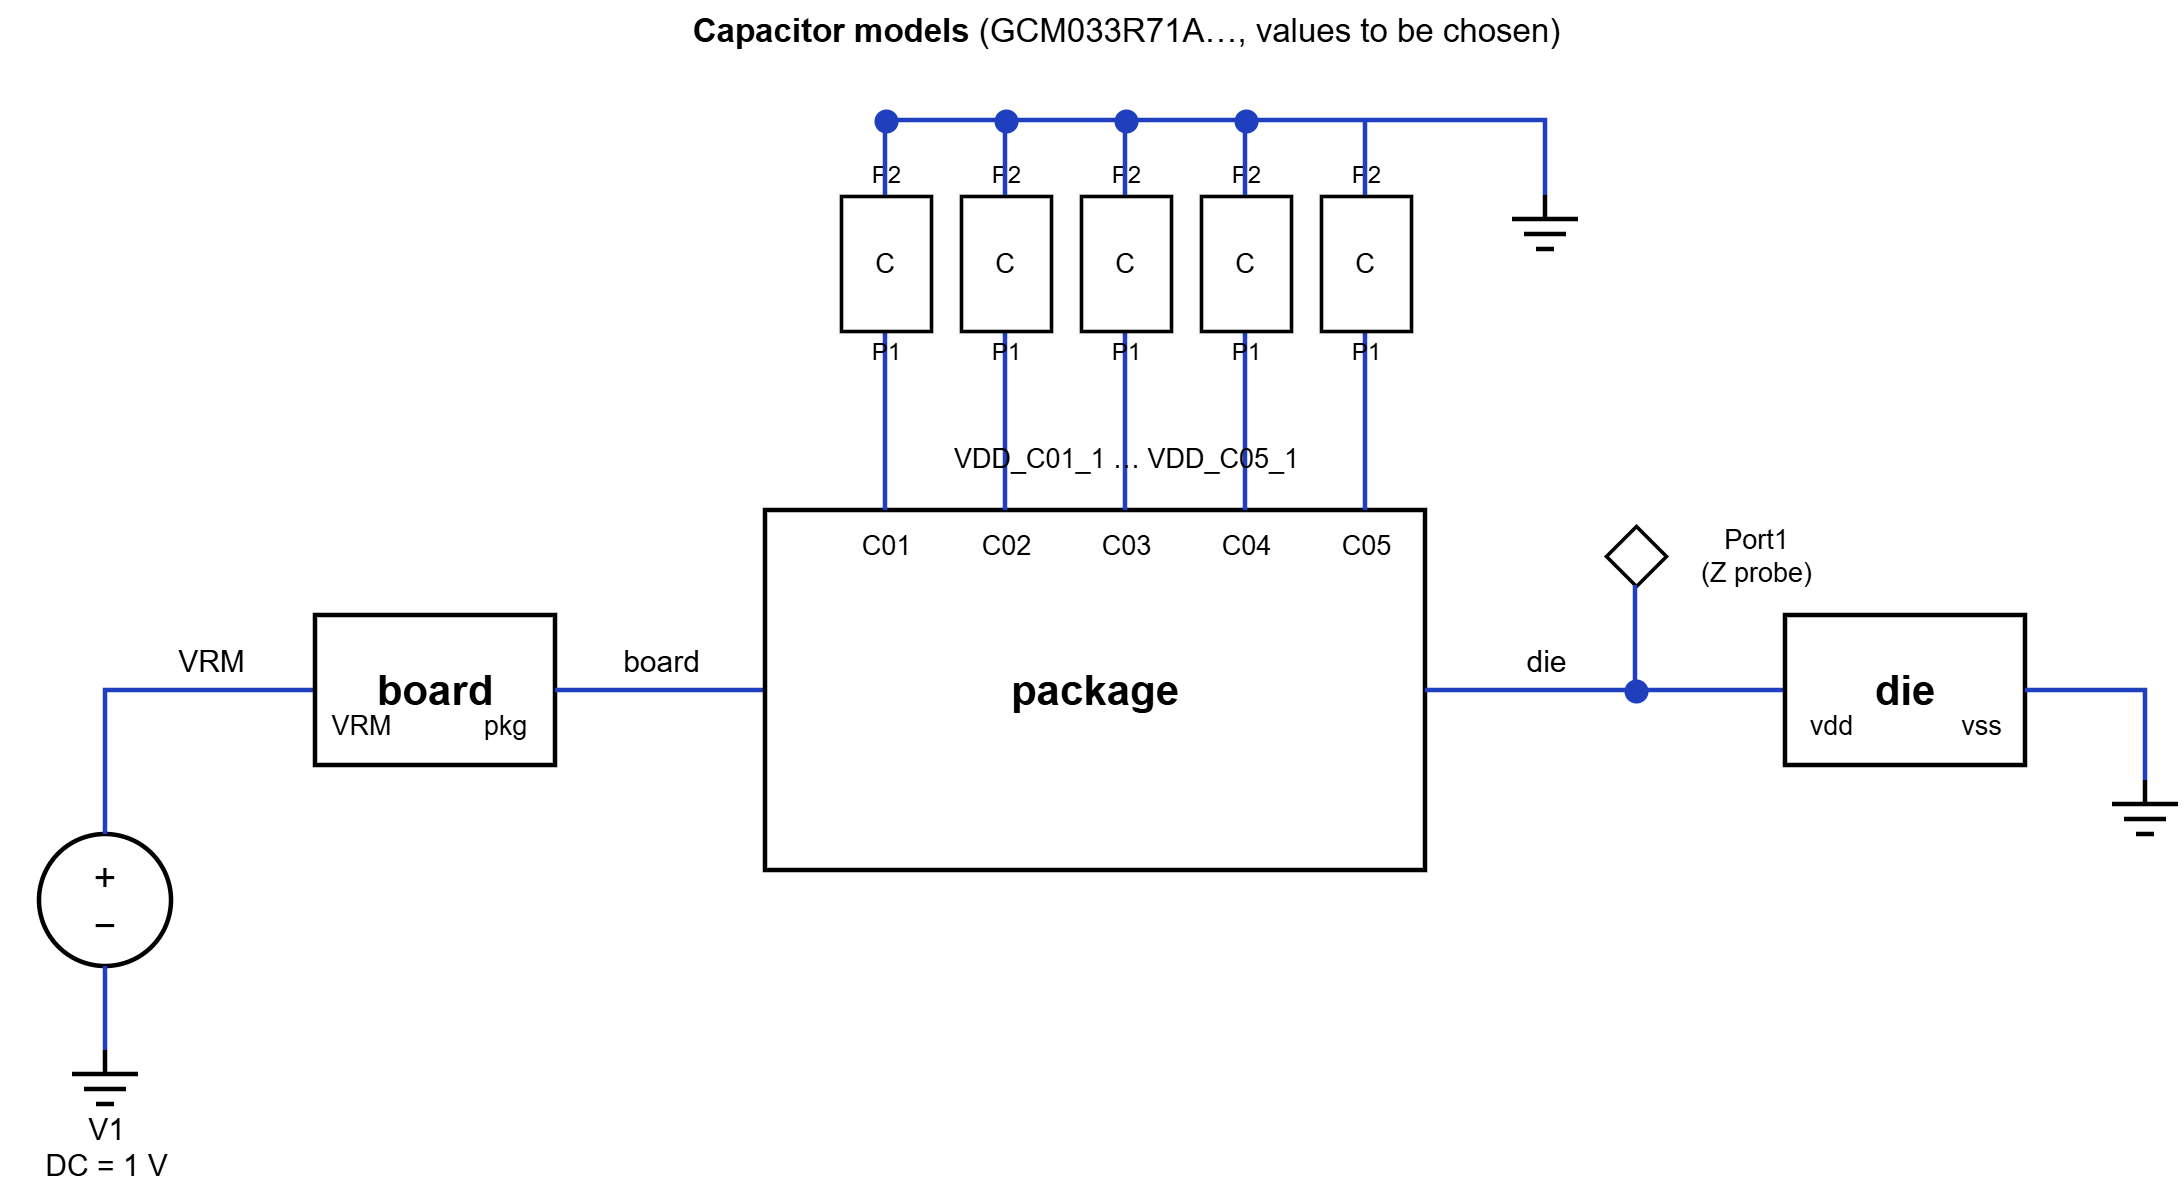
\includegraphics[width=0.95\textwidth]{./eser1/pdn_schematic.png}
\caption{Scheme of the complete PDN: ideal 1~V VRM, board, package and die. The five ports of the package on the capacitor locations (C01--C05) are left open in the PDN without decoupling capacitors.}
\label{fig:pdn}
\end{figure}

\noindent The part of the netlist that instantiates and connects the modules is shown in Listing~\ref{lst:pdn_inst}.

\begin{lstlisting}[language={ltspice}, caption={Instances and connection of the modules in the netlist \texttt{pdn.cir}.}, label={lst:pdn_inst}]
* ---- Supply: ideal VRM, 1 V DC ----
VVRM vrm 0 DC 1

* ---- Board: port 1 (VRM) on the source, port 2 (package) towards the package ----
* pin order: a_1 b_1 a_2 b_2
Xboard vrm 0 pkg_board 0 board_passive

* ---- Package ----
* pin order: a_1 b_1 ... a_7 b_7
*   1..5 = capacitor locations C01..C05
*   6    = board side (connected to board port 2)
*   7    = die side   (vdie)
Xpkg c01 0 c02 0 c03 0 c04 0 c05 0 pkg_board 0 vdie 0 package_ports_on_caps_passive

* ---- Die: VDD on node vdie, VSS on ground ----
Xdie vdie 0 die_model
\end{lstlisting}


% eser 2
\section{Exercise 2: PDN impedance in the frequency domain}

%%%%%%%%%%%%%%%%%%%%%%%%%%%%%%%%%%%%%%%%%%%%%%%%%%%%%%%%%%%

\subsection{AC analysis of the PDN}

To compute the impedance of the PDN seen from the die interface, a very simple netlist, \texttt{pdn\_ac.cir}, has been written. It includes the
complete netlist \texttt{pdn.cir} created in the previous exercise, so that the PDN is exactly the same one (without decoupling capacitors), and it
adds only the excitation and the analysis directive.

\noindent\\ The impedance is obtained with a \textit{test current}: an AC current source of $1\,\text{A}$ is connected to the node \texttt{vdie}, which
is the die interface (the port where the impedance is requested).\\ By definition, the impedance seen from a port is the ratio between the voltage across
the port and the current entering it:
\begin{equation}
  Z(f) = \frac{V(f)}{I(f)}\,
\end{equation}
\noindent\\ Since the injected current has a magnitude of $1\,\text{A}$, the voltage at \texttt{vdie} is numerically equal to the impedance:
$Z(f) = V(\texttt{vdie})/1\,\text{A}$. The other sources do not affect the result: in an AC analysis the ideal $1\,\text{V}$ source of the VRM behaves
as a short circuit, and the PWL current load of the die has no AC magnitude, so it does not contribute. The only excitation is therefore the test
current, and the analysis describes the passive network alone.

\noindent\\ The AC analysis is performed from $1\,\text{Hz}$ to $5\,\text{GHz}$, with a logarithmic sweep of 1000 points per decade. The corresponding
part of the netlist is shown in \autoref{lst:pdn_ac}, while the plot of $|Z|$ obtained with LTspice is shown in \autoref{fig:zdie_nodecaps}.

\begin{lstlisting}[language=ltspice, caption={Netlist \texttt{pdn\_ac.cir} used for the AC analysis.}, label={lst:pdn_ac}]
.include "../eser1/pdn.cir"

* AC test current into the die node (the "Port1" of the slide schematic)
Iac 0 vdie DC 0 AC 1
.ac dec 1000 1 5G
.meas ac zmax MAX mag(V(vdie))
.meas ac fpk  WHEN mag(V(vdie))=zmax
.meas ac z100M FIND mag(V(vdie)) at 100Meg
.end
\end{lstlisting}

\begin{figure}[!h]
\centering
% Replace the placeholder below with the LTspice plot:
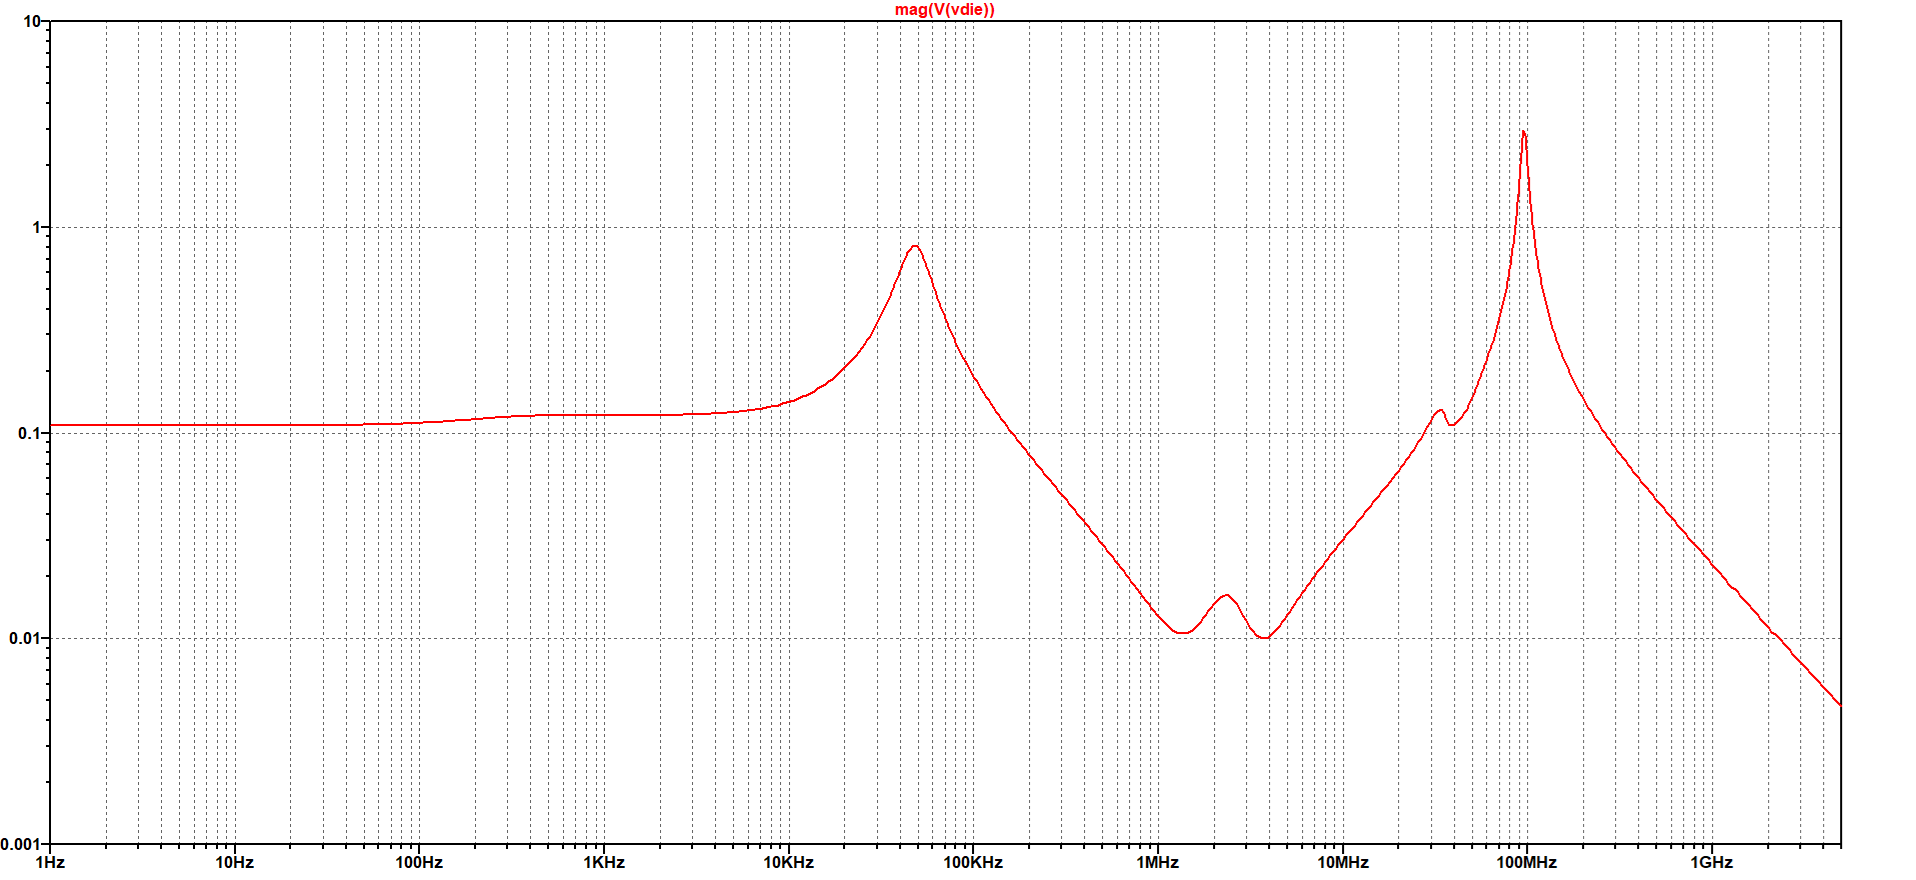
\includegraphics[width=0.95\textwidth]{./eser2/pdn_ac.png}
%\fbox{\parbox{0.9\textwidth}{\centering\vspace{3cm} Figure placeholder: LTspice plot of $|Z|$ at the die port, without decoupling capacitors\vspace{3cm}}}
\caption{Impedance magnitude seen from the die interface (node \texttt{vdie}) of the PDN without decoupling capacitors, from $1\,\text{Hz}$ to $5\,\text{GHz}$.}
\label{fig:zdie_nodecaps}
\end{figure}

\noindent From the Figure reported above, it is possible to see that the impedance
reaches the peak value of $|Z|_{\max} \approx 3~\Omega$ at the frequency $f_{\text{peak}} = 96~\text{MHz}$,
in line with the expected behaviour of the PDN. Moreover, exploiting the \texttt{.meas} statements in the netlist,
LTspice automatically computes the peak value and the corresponding frequency, which are reported in the log file \texttt{pdn\_ac.log}.
\\ The values reported in the log file are:
\[
|Z|_{\max} = 3.057~\Omega, \quad f_{\text{peak}} = 95.94~\text{MHz}
\]

%%%%%%%%%%%%%%%%%%%%%%%%%%%%%%%%%%%%%%%%%%%%%%%%%%%%%%%%%%%
\newpage
\subsection{Choice of the frequency range}

The upper limit of the sweep, $5\,\text{GHz}$, is set by the bandwidth of the models. The board and the package macromodels have been obtained
from S-parameter data, \texttt{board.ts} for the board and \texttt{package\_ports\_on\_caps.ts} for the package, that cover a limited frequency range,
and a rational macromodel is reliable only inside the range of the data it was fitted to. In particular:
\begin{itemize}
  \item the board model has been fitted over a bandwidth of $5\,\text{GHz}$ (as stated in the header of \texttt{board\_passive.cir});
  \item the package model has been fitted over a bandwidth of $10\,\text{GHz}$ (as stated in the header of the package macromodel file);
  \item the die model is a lumped RC network, and it has no frequency limit of its own.
\end{itemize}
The validity of the whole PDN is therefore limited by the narrowest model, the board, and this is why the analysis stops at $5\,\text{GHz}$. Above
this frequency the simulator still returns numbers, but they are only an extrapolation of the models, and they would not be a trustworthy
description of the real network. Moreover, the reference curve shown in the assignment also stops at about $5\,\text{GHz}$.

\noindent\\ The lower limit of $1\,\text{Hz}$ has been chosen to include the whole behaviour of the network, down to the region where the impedance
no longer changes: at the lowest frequencies it is flat and equal to the DC resistance of the PDN. The S-parameter data start from DC, so the models
are valid there, and extending the sweep downwards has a negligible cost, since the whole analysis takes less than a second.

% eser 3
\section{Exercise 3: Stand-alone capacitor impedance poltting and validation}

%%%%%%%%%%%%%%%%%%%%%%%%%%%%%%%%%%%%%%%%%%%%%%%%%%%%%%%%%%%

\subsection{Extraction of capacitor impedance from vendor S-parameters}

The stand-alone impedance of the six candidate capacitors has been characterised in MATLAB starting from frequency-domain measurements given by the vendor.\\
The data are provided in the IdEM workspace \texttt{capacitors\_workspace.idem.mat}, which contains the MATLAB structure \texttt{idemws}. 
Its field \texttt{idemws.DUM} is a $6 \times 1$ cell array, one entry per capacitor, each storing:
\begin{itemize}
    \item  Part name, 
    \item  Vector of 401 logarithmically spaced frequency points,
    \item  The S-parameter matrix for each frequency point, stored as a $2 \times 2$ cell array of complex vectors,
    \item  The reference impedance $R_0 = 50~\Omega$.
\end{itemize}

The core extraction loop of the MATLAB script \texttt{cap\_impedance\_matlab.m} is shown below.

\begin{lstlisting}[language=Matlab, caption={Extraction of the stand-alone capacitor impedance from vendor S-parameters in \texttt{cap\_impedance\_matlab.m}.}, label={lst:capzextract}]
for k = 1:N
    D       = idemws.DUM{k};
    name{k} = D.Name;
    f{k}    = D.f(:);
    S21     = D.S{2,1}(:);
    Z{k}    = 2*D.R0*(1 - S21) ./ S21;
    C_nF(k) = str2double(D.Name(11:12)) * 10^str2double(D.Name(13)) * 1e-3;
end
\end{lstlisting}

\noindent The vendor characterised each component in \textit{series mode}, placing the capacitor in series between port~1 and port~2 of a two-port $R_0 = 50~\Omega$ measurement setup.\\
Under this configuration, the transmission parameter $S_{21}$ is related to the series impedance $Z$ of the capacitor by
\begin{equation}
    S_{21} = \frac{2 R_0}{Z + 2 R_0} \quad \Longrightarrow \quad Z = 2 R_0 \frac{1 - S_{21}}{S_{21}}.
    \label{eq:s21toz}
\end{equation}

\noindent For each component, the nominal capacitance in nF is also automatically decoded from the capacitor part number.\\


\noindent The resulting impedance magnitudes $|Z(f)|$ are plotted on a log--log scale from $0.1~\text{MHz}$ to $10~\text{GHz}$ in \ref{fig:capzvendor}. 
As expected for real decoupling capacitors, each curve exhibits a capacitive behaviour ($|Z| \propto 1/f$) at low frequency, reaches a minimum $|Z|_{\min}$ (corresponding to the equivalent series resistance, ESR) at its self-resonance frequency $f_{\text{SRF}}$, 
and becomes inductive ($|Z| \propto f$) above $f_{\text{SRF}}$ due to the equivalent series inductance (ESL).

\begin{figure}[!h]
\centering
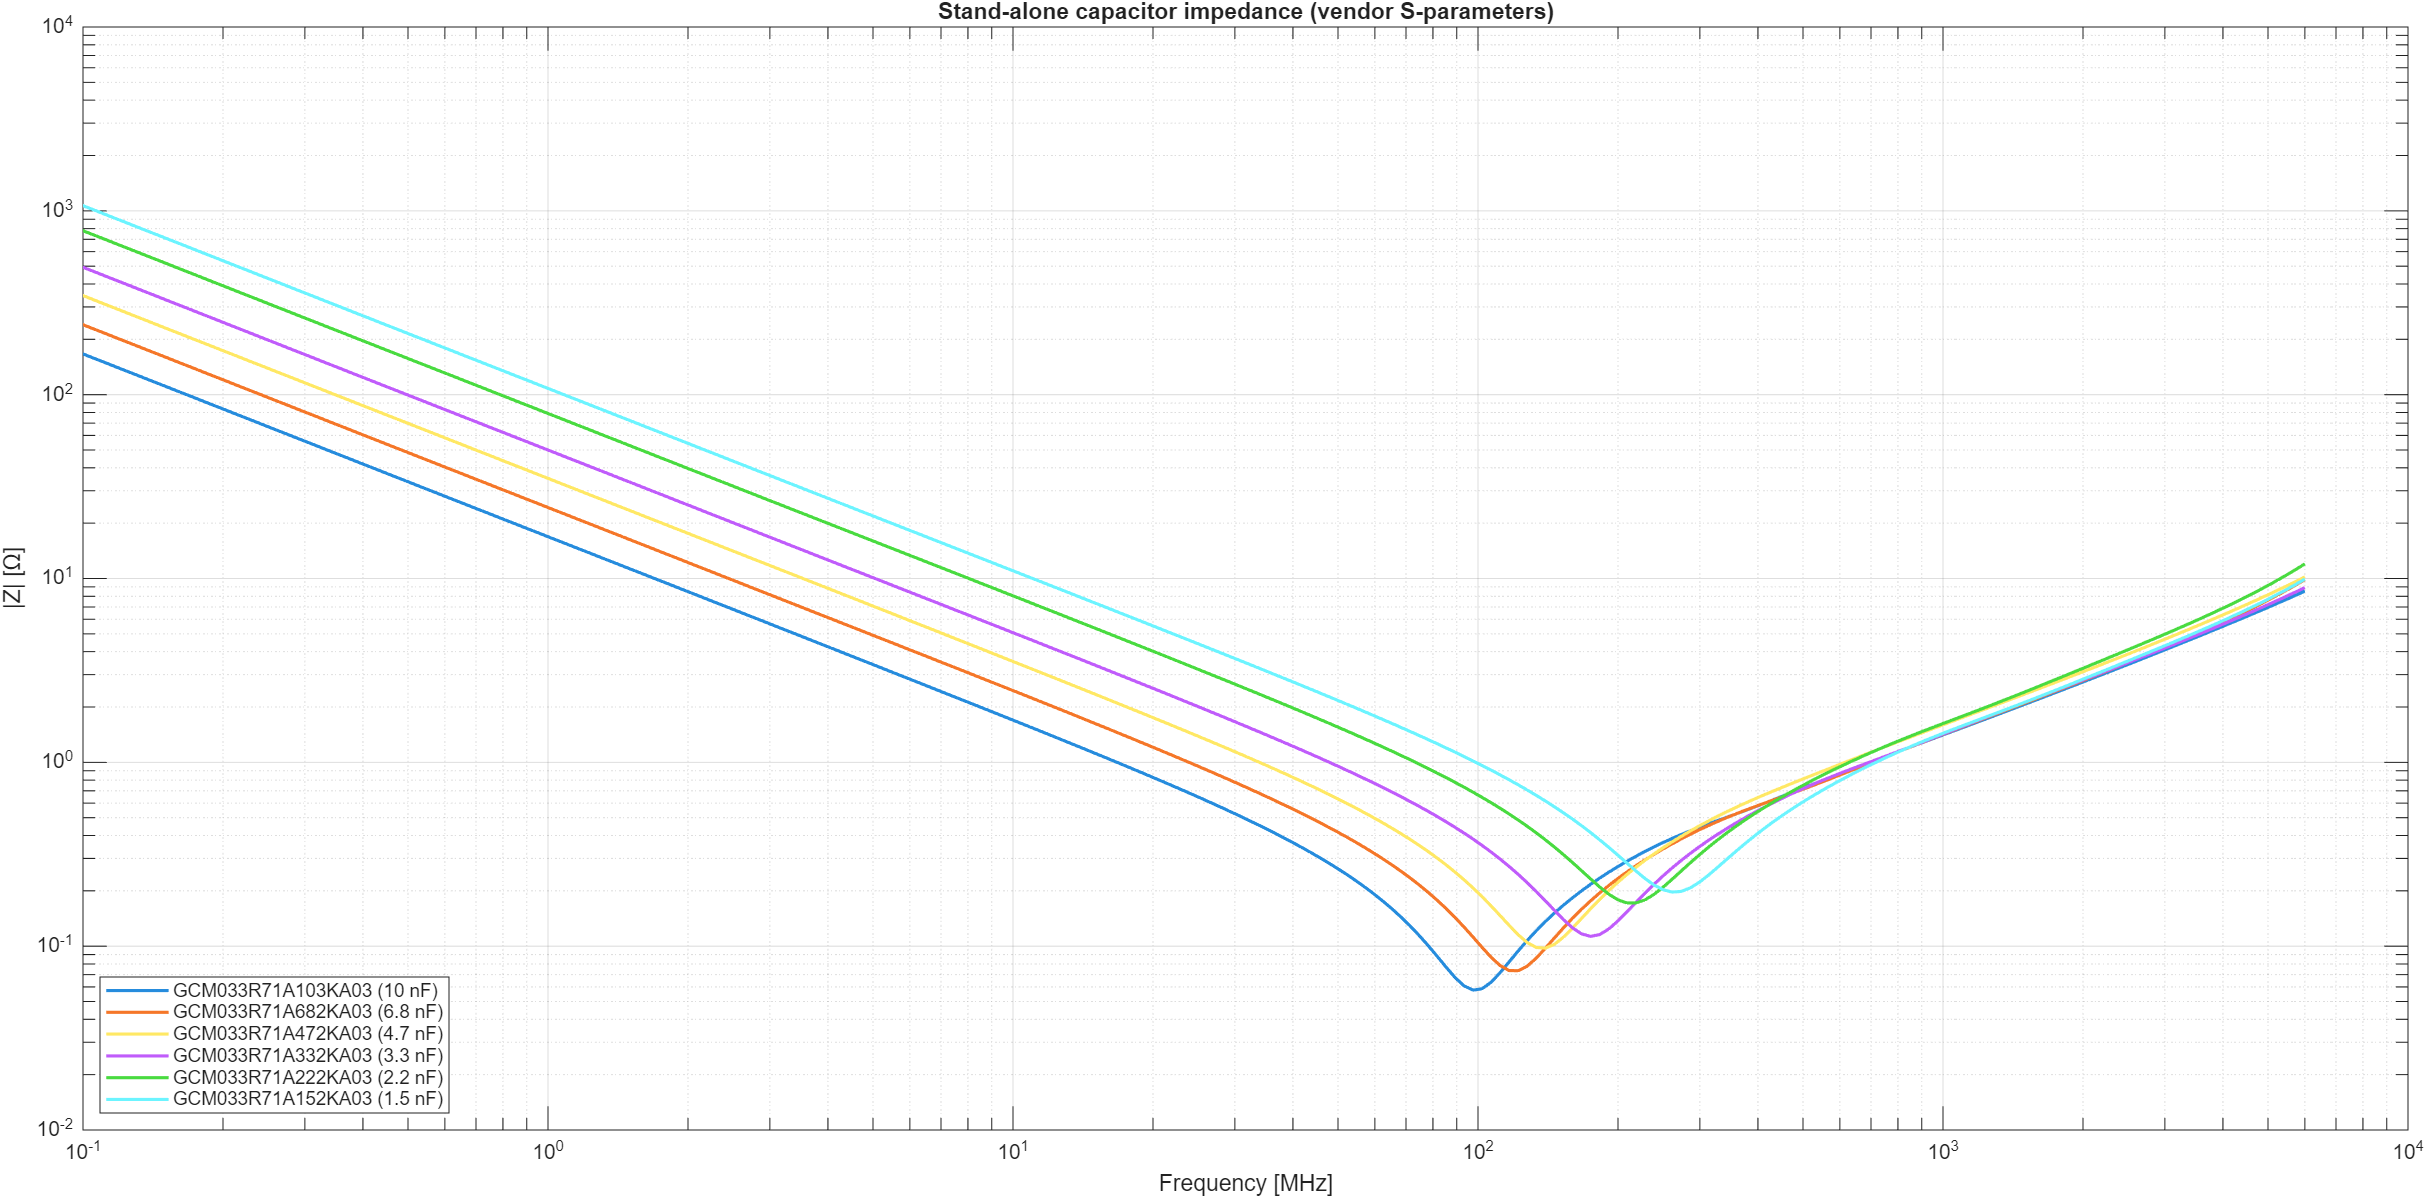
\includegraphics[width=0.7\textwidth]{./eser3/Images/caps.png}
\caption{Stand-alone impedance magnitude $|Z(f)|$ of the six Murata decoupling capacitors extracted from the vendor S-parameters.}
\label{fig:capzvendor}
\end{figure}

\noindent Table~\ref{tab:cap_srf} summarises the nominal capacitance, self-resonance frequency $f_{\text{SRF}}$, and minimum impedance $|Z|_{\min}$ extracted on the vendor frequency grid. It should be noted that the vendor grid consists of 401 logarithmically spaced points (approximately $4.6\%$ spacing per step), which sets the resolution limit on the extracted $f_{\text{SRF}}$ values. Finally, the extracted data (\texttt{f}, \texttt{Z}, \texttt{name}, \texttt{C\_nF}) are saved to \texttt{cap\_Z\_vendor\_data.mat} for the subsequent SPICE validation.

\begin{table}[!h]
\centering
\caption{Nominal capacitance, self-resonance frequency, and minimum impedance of the six capacitors extracted from vendor S-parameters.}
\label{tab:cap_srf}
\begin{tabular}{lccc}
\hline
\textbf{Part number} & \textbf{$C$ [nF]} & \textbf{$f_{\text{SRF}}$ [MHz]} & \textbf{$|Z|_{\min}$ [$\Omega$]} \\
\hline
\texttt{GCM033R71A103KA03} & 10.0 &  97.54 & 0.0577 \\
\texttt{GCM033R71A682KA03} &  6.8 & 122.01 & 0.0735 \\
\texttt{GCM033R71A472KA03} &  4.7 & 139.55 & 0.0976 \\
\texttt{GCM033R71A332KA03} &  3.3 & 174.57 & 0.1131 \\
\texttt{GCM033R71A222KA03} &  2.2 & 218.37 & 0.1717 \\
\texttt{GCM033R71A152KA03} &  1.5 & 261.20 & 0.1970 \\
\hline
\end{tabular}
\end{table}

%%%%%%%%%%%%%%%%%%%%%%%%%%%%%%%%%%%%%%%%%%%%%%%%%%%%%%%%%%%

\subsection{Validation of the vendor SPICE models}

To verify that the SPICE subcircuit models provided by the vendor accurately reproduce the measured frequency-domain behaviour, 
an AC simulation has been performed in LTspice on a testbench netlist (\texttt{caps\_spice\_ac.cir}) containing the six capacitor models driven by unit AC current sources, 
so that each node voltage directly equals the capacitor impedance $Z(f)$. 
The simulated node voltages (\texttt{V(zXXX)}, where \texttt{XXX} is the three-digit capacitance code) have been exported from LTspice as a text file (\texttt{caps\_spice\_ac.txt}).
\noindent Because the SPICE simulation and the vendor S-parameters may be defined on different frequency grids, the comparison is restricted to the overlapping frequency range and the SPICE response is interpolated onto the vendor frequency points:
The relative magnitude error is computed as
    \begin{equation}
        \varepsilon_{|Z|}(f) = \frac{\big||Z_{\text{SPICE}}(f)| - |Z_{\text{vendor}}(f)|\big|}{|Z_{\text{vendor}}(f)|} \times 100\%;
    \end{equation}

\begin{figure}[!h]
\centering
 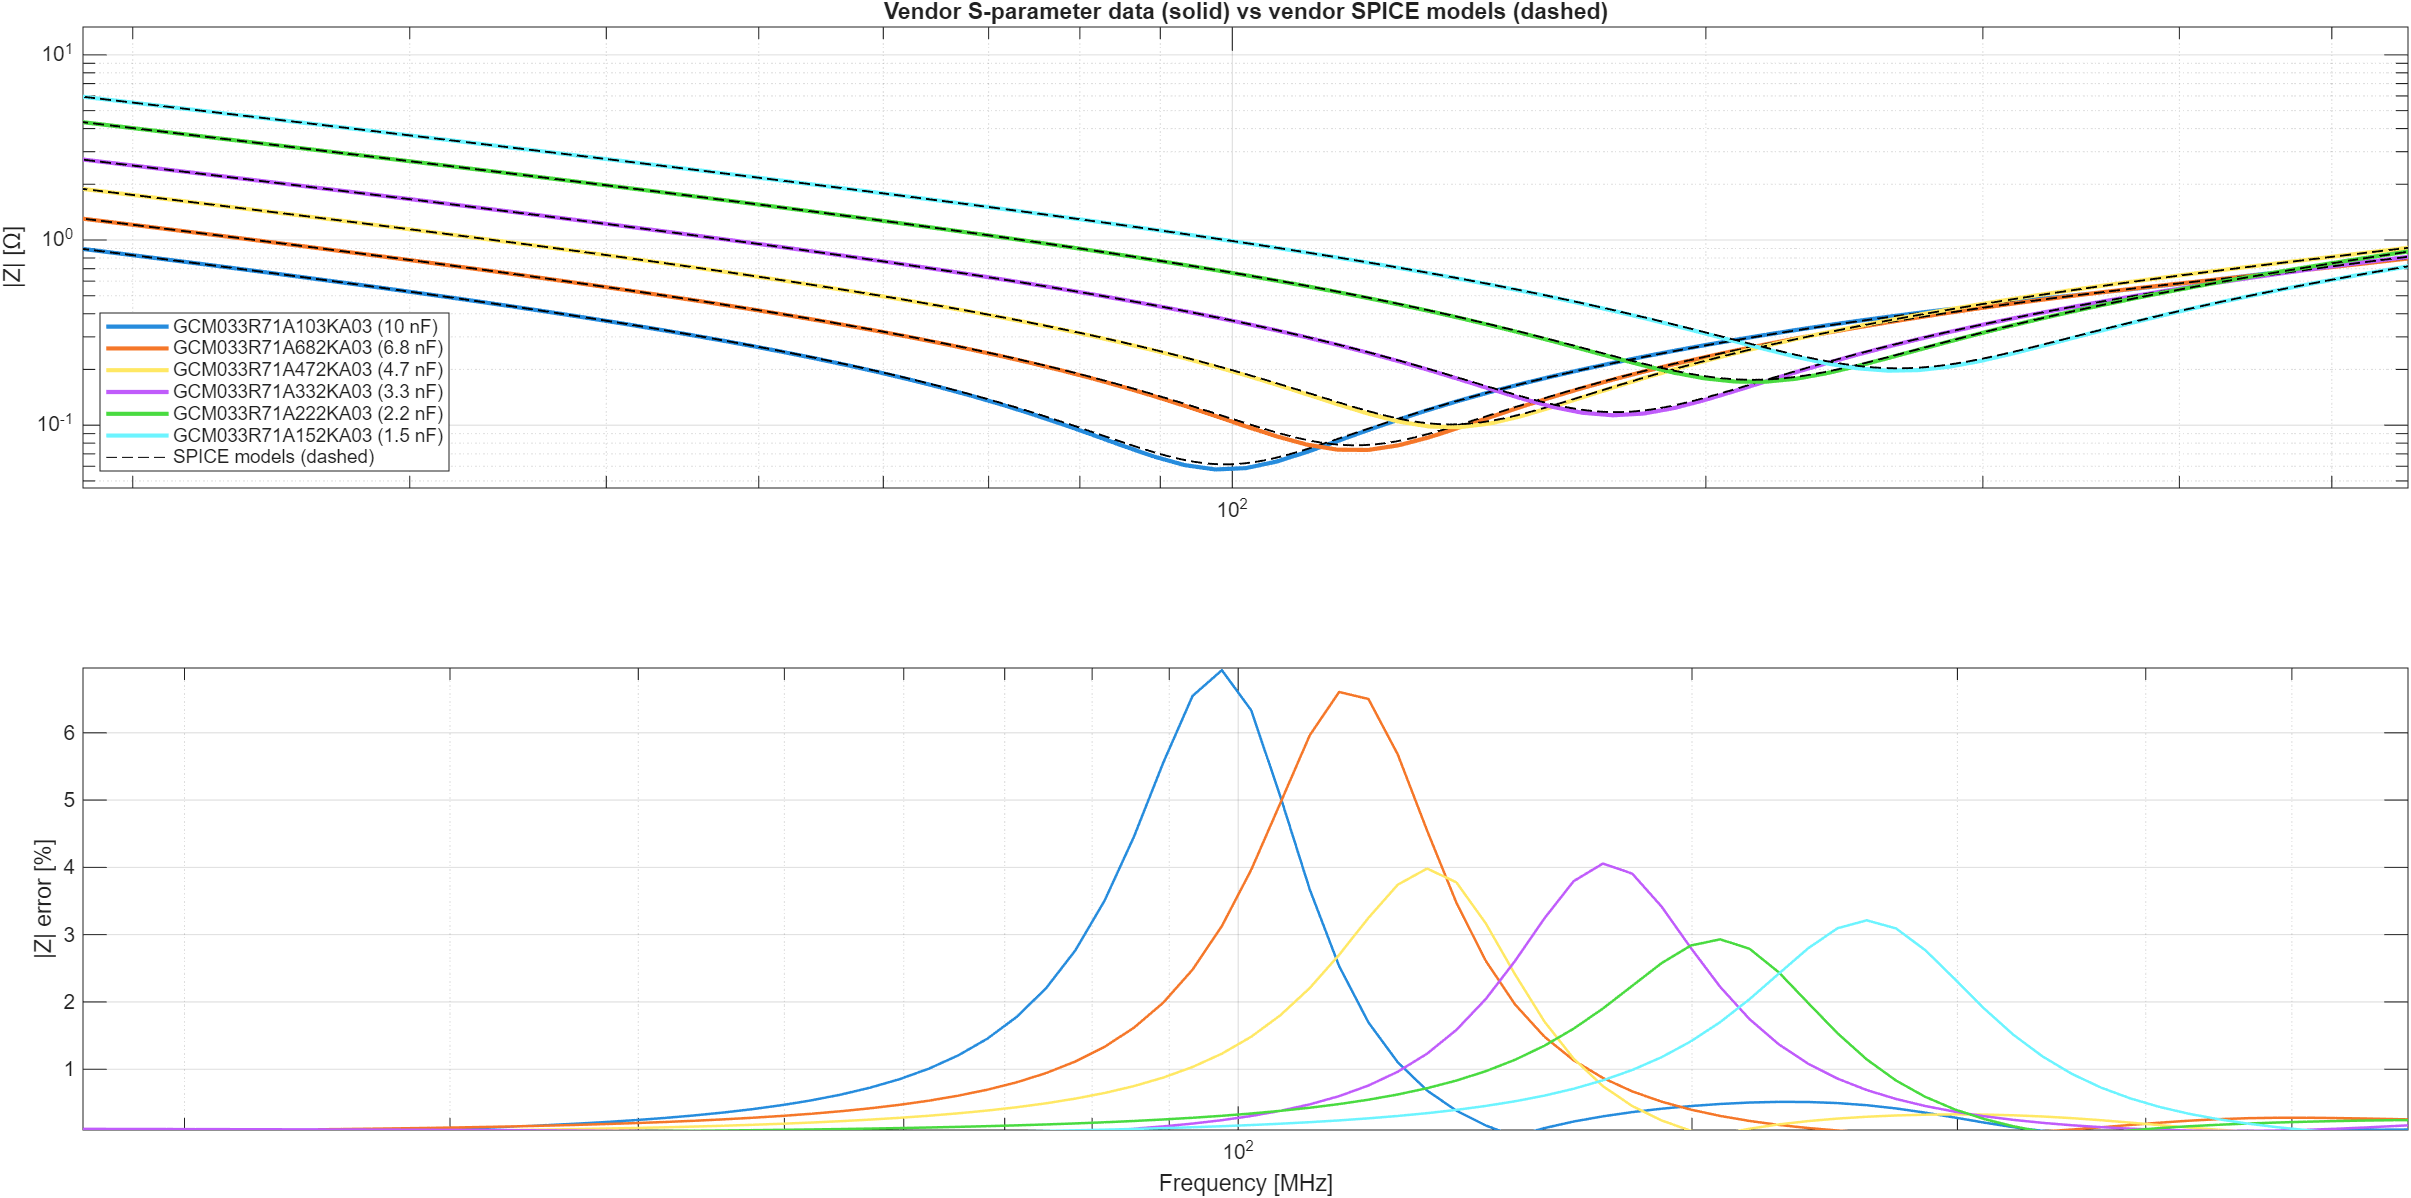
\includegraphics[width=0.92\textwidth]{./eser3/Images/cap_val.png}
\caption{Validation of the vendor SPICE models against the vendor S-parameter data. Top: impedance magnitude $|Z(f)|$ from vendor S-parameters (solid lines) and SPICE AC simulation (dashed black lines). Bottom: relative magnitude error $\varepsilon_{|Z|}$ versus frequency.}
\label{fig:capspiceval}
\end{figure}

\noindent The visual comparison between the vendor S-parameter curves and the SPICE simulations show a loss of accracy near the self-resonance frequency. 
This is confirmed by the relative magnitude error which peaks at the self-resonance frequency and is higher for bigger capacitors.

\begin{table}[!h]
\centering
\caption{Maximum impedance magnitude  between vendor S-parameters and vendor SPICE models.}
\label{tab:cap_val_err}
\begin{tabular}{lccc}
\hline
\textbf{Part number} & \textbf{Max $|Z|$ error [\%]} & \textbf{Frequency [MHz]} \\
\hline
\texttt{GCM033R71A103KA03} & 6.930 &  97.54   \\
\texttt{GCM033R71A682KA03} & 6.606 & 116.67   \\
\texttt{GCM033R71A472KA03} & 3.982 & 133.44   \\
\texttt{GCM033R71A332KA03} & 4.057 & 174.57   \\
\texttt{GCM033R71A222KA03} & 2.931 & 208.81   \\
\texttt{GCM033R71A152KA03} & 3.213 & 261.20   \\
\hline
\end{tabular}
\end{table}

\noindent Overall, the SPICE models show good agreement with the vendor S-parameter data across the frequency band of interest, 
confirming that they can be reliably used in the PDN simulations of the following exercises.

% eser 4
\section{Exercise 4: Transient analysis of the PDN without decoupling capacitors}

%%%%%%%%%%%%%%%%%%%%%%%%%%%%%%%%%%%%%%%%%%%%%%%%%%%%%%%%%%%

In this exercise the PDN without decoupling capacitors is simulated in the time domain, with the die drawing the supplied current, and the voltage
ripple at the die interface (node \texttt{vdie}) is evaluated. This is the reference case: in Exercise~5 the different decap configurations are
going to be compared with this result.

\noindent\\ The simulation uses the netlist \texttt{pdn\_tran.cir} (\autoref{lst:pdn_tran}). It simply includes the PDN of Exercise~1, so the VRM is still
the ideal 1~V source and the load is the PWL current source of the die model. 
The die current, already described in Exercise~1, is a PWL waveform
that varies between about 21 and 287~mA, with an average value of about
109~mA. It is made of current pulses repeated every 10~ns, so the
activity of the die is at 100~MHz.
One full period of the current is simulated, 12~$\mu$s, with a
maximum time step of 72~ps, the same step of the PWL data, otherwise LTspice could skip some points of the current.
To keep the output file small
only \texttt{V(vdie)} is saved, and a \texttt{.meas} statement gives the peak-to-peak value directly from LTspice.

\begin{lstlisting}[language={ltspice}, caption={Netlist \texttt{pdn\_tran.cir} used for the transient analysis.}, label={lst:pdn_tran}]
.include "../eser1/pdn.cir"
.save V(vdie)
.tran 72p 12u 0 72p
.meas tran vpp PP V(vdie)
.meas tran vpp_ss PP V(vdie) FROM=0.5u TO=12u
.end
\end{lstlisting}

\noindent The simulation takes about 3 minutes. This already shows that running a transient simulation for every decap configuration in Exercise~5 is not
a realistic option.

\noindent The voltage at the die over the whole simulation is shown in \autoref{fig:vdie_time}, and the main values are collected in \autoref{tab:ripple}.

\begin{figure}[h]
  \centering
  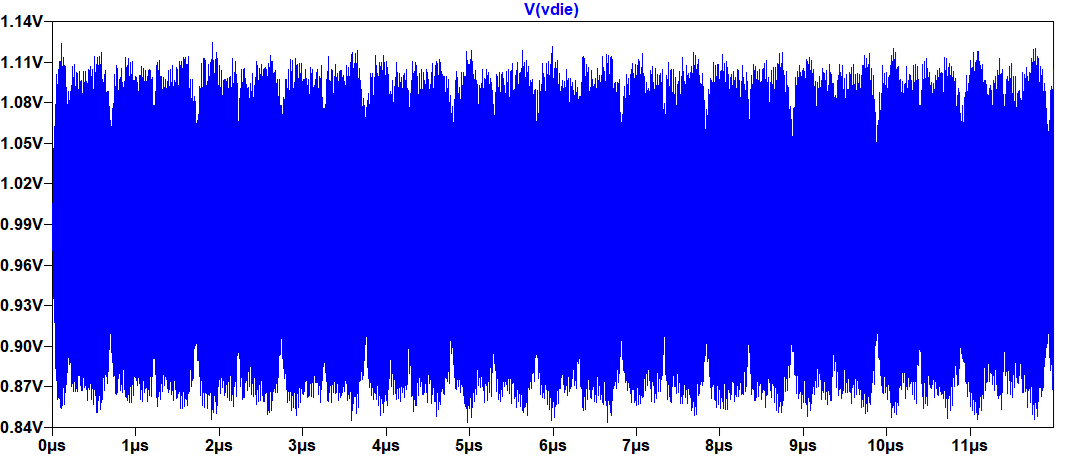
\includegraphics[width=\textwidth]{./eser4/vdie_time.png}
  \caption{Voltage at the die interface without decoupling capacitors over the whole simulation (12~$\mu$s).}
  \label{fig:vdie_time}
\end{figure}

\begin{table}[h]
  \centering
  \begin{tabular}{|l|c|}
    \hline
    \textbf{Quantity} & \textbf{Value} (full) \\
    \hline
    Peak-to-peak ripple (LTspice \texttt{.meas}) & 280.8~mV  \\
    Minimum voltage                              & 0.844~V   \\
    Maximum voltage                              & 1.125~V   \\
    Average voltage                              & 0.986~V   \\
    \hline
  \end{tabular}
  \caption{Voltage ripple at the die interface without decoupling capacitors.}
  \label{tab:ripple}
\end{table}

\noindent The ripple is really large: 281~mV peak-to-peak, which is 28\% of the supply voltage. The minimum is 0.844~V and the maximum is
1.125~V, so the voltage goes well outside a typical $\pm 5\%$ tolerance band, and this happens over the whole simulation, not only in a few
points. One could expect mainly a voltage drop, but the voltage actually goes both below and above 1~V, almost symmetrically. The average value
is 0.986~V: the 14~mV of difference from 1~V, with an average current of 109~mA, is the static drop on the DC resistance of the PDN.

\noindent\\ \autoref{fig:vdie_zoom} shows a zoom of 100~ns around the minimum of the voltage. Here the voltage looks almost like a sinusoid with a period of
10~ns, i.e.\ at 100~MHz, the same frequency of the activity of the die. The voltage does not follow each current pulse separately: the
oscillation grows over several cycles, which is the typical behaviour of a resonant circuit excited at its resonance frequency.

% FIGURE 2 - LTspice: same plot as Figure 1, click on the numbers of the time axis and set
% Left = 4.9u, Right = 5u (Y axis can stay 0.8-1.2 V). Export as latex/eser4/vdie_zoom.png
\begin{figure}[h]
  \centering
  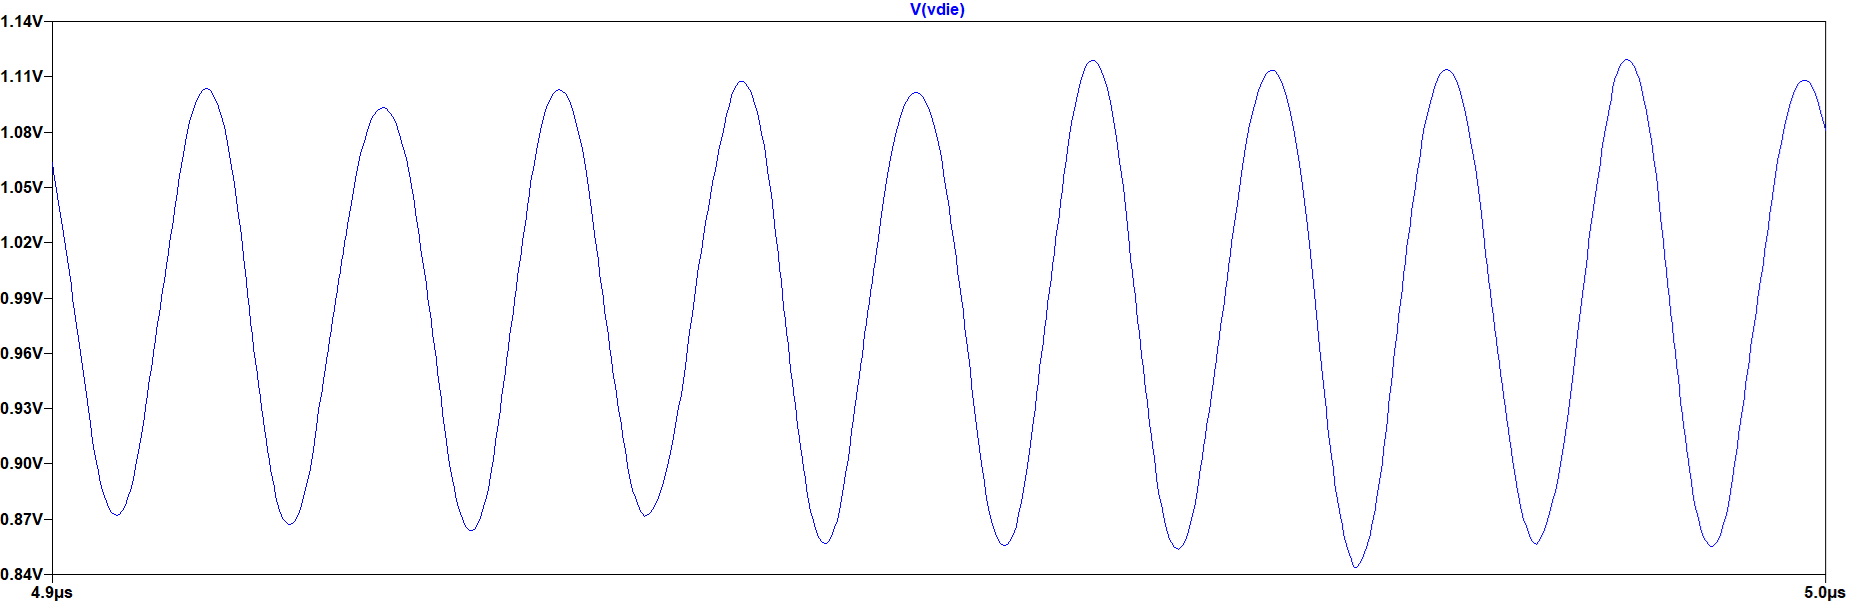
\includegraphics[width=\textwidth]{./eser4/vdie_zoom.png}
  \caption{Zoom of the voltage at the die interface over 100~ns, around the minimum of the voltage.}
  \label{fig:vdie_zoom}
\end{figure}



\noindent This is consistent with the result of Exercise~2: the impedance of the PDN
seen from the die has its main peak at about 96~MHz ($3.06~\Omega$), and at
100~MHz, the frequency of the main component of the die current, it is
still about $2.0~\Omega$.
The peak-to-peak ripple obtained in this work, about 281~mV, is higher than
the reference value of about 250~mV provided. This
difference is consistent with the result of Exercise~2: the maximum of the
PDN impedance obtained here is about $3.06~\Omega$, while the reference
value is about $2.9~\Omega$. Since the ripple is mainly caused by the die
current at the resonance of the PDN, a higher impedance peak produces a
proportionally higher ripple: both values are about 10\% higher
than the reference ones. The ripple is also confirmed by the
frequency-domain method of Exercise~5, which gives 282.2~mV without
decoupling capacitors.
So the problem is not the current itself, but the fact that its main component falls exactly on the resonance peak of the PDN. This also shows
what the decoupling capacitors have to do in Exercise~5: reduce the impedance at 100~MHz, or move the resonance away from the main frequency of the
die current.

% eser 5
\section{Exercise 5: Optimization of the decoupling capacitors}

In this last exercise the five decoupling capacitors are connected to the package, and their values are chosen to minimise the peak-to-peak voltage ripple at the
die interface. Each of the five locations (C01--C05) can host one of the six vendor capacitors (1.5, 2.2, 3.3, 4.7, 6.8 and 10~nF), so there are
$6^5 = 7776$ possible configurations. Since a single transient simulation of the PDN takes about three minutes (Exercise~4), simulating all of them would require
more than two weeks. For this reason the problem is solved with a semi-analytical method: the PDN is characterised only once with a few AC
simulations, and the effect of any configuration of capacitors is then computed with simple matrix algebra.

%%%%%%%%%%%%%%%%%%%%%%%%%%%%%%%%%%%%%%%%%%%%%%%%%%%%%%%%%%%

\subsection{Impedance and voltage ripple with decoupling capacitors}
\label{sec:theory}

The PDN without decoupling capacitors, seen from the five capacitor locations and from the die, is a linear network with six ports: the ports $1,\dots,5$ at
the capacitor locations (C01--C05) and the port $d$ at the die interface. In the frequency domain, the network is described by its $6\times 6$ impedance matrix
$\mathbf{Z}(f)$, which links the port voltages to the port currents (all the currents flow \textit{into} the network):
\begin{equation}
  \begin{bmatrix} \mathbf{V}_c \\ V_d \end{bmatrix} =
  \begin{bmatrix} \mathbf{Z}_{cc} & \mathbf{Z}_{cd} \\ \mathbf{Z}_{dc} & Z_{dd} \end{bmatrix}
  \begin{bmatrix} \mathbf{I}_c \\ I_d \end{bmatrix},
  \label{eq:zmatrix}
\end{equation}
where $\mathbf{V}_c$ and $\mathbf{I}_c$ are the $5\times 1$ vectors of the voltages and of the currents at the capacitor ports, $\mathbf{Z}_{cc}$ is the
$5\times 5$ block between the capacitor ports, $\mathbf{Z}_{cd}$ and $\mathbf{Z}_{dc}$ are the $5\times 1$ and $1\times 5$ blocks that couple the capacitor
ports with the die port, and $Z_{dd}$ is the impedance seen from the die port when no capacitor is connected. The matrix is the one of the whole PDN, with the
VRM modelled as an ideal voltage source, which is a short circuit for the AC components, and with the passive RC network of the die.
Written out, the matrix equation \eqref{eq:zmatrix} becomes
\begin{align}
  \mathbf{V}_c &= \mathbf{Z}_{cc}\,\mathbf{I}_c + \mathbf{Z}_{cd}\,I_d, \label{eq:vc}\\
  V_d &= \mathbf{Z}_{dc}\,\mathbf{I}_c + Z_{dd}\,I_d. \label{eq:vd}
\end{align}

\noindent\\ When the capacitors are connected, each of them is a one-port connected between the capacitor port and the ground. The current that enters
the network is the opposite of the current that enters the capacitor, so that
\begin{equation}
  \mathbf{V}_c = -\mathbf{Z}_{cap}\,\mathbf{I}_c,
  \qquad
  \mathbf{Z}_{cap} = \mathrm{diag}\big(Z_{C_1}(f),\dots,Z_{C_5}(f)\big),
  \label{eq:cap}
\end{equation}
where $Z_{C_i}(f)$ is the impedance of the capacitor mounted on the location $i$, that is one of the six vendor models. Replacing \eqref{eq:cap} in
\eqref{eq:vc} gives
\begin{equation}
  -\mathbf{Z}_{cap}\,\mathbf{I}_c = \mathbf{Z}_{cc}\,\mathbf{I}_c + \mathbf{Z}_{cd}\,I_d
  \;\Longrightarrow\;
  \mathbf{I}_c = -\big(\mathbf{Z}_{cc} + \mathbf{Z}_{cap}\big)^{-1}\mathbf{Z}_{cd}\,I_d,
\end{equation}
which describes how the current injected at the die port is shared between the capacitors. Replacing this expression of $\mathbf{I}_c$ in \eqref{eq:vd}, the voltage
at the die port is
\begin{equation}
  V_d = \Big[ Z_{dd} - \mathbf{Z}_{dc}\big(\mathbf{Z}_{cc} + \mathbf{Z}_{cap}\big)^{-1}\mathbf{Z}_{cd} \Big] I_d ,
\end{equation}
and the impedance seen from the die with the decoupling capacitors, $Z_{die} = V_d/I_d$, is
\begin{equation}
  \boxed{\,Z_{die}(f) = Z_{dd}(f) - \mathbf{Z}_{dc}(f)\,\big[\mathbf{Z}_{cc}(f) + \mathbf{Z}_{cap}(f)\big]^{-1}\,\mathbf{Z}_{cd}(f)\,}
  \label{eq:zdie}
\end{equation}
This expression has the expected limits: if the capacitors are removed ($\mathbf{Z}_{cap}\to\infty$) the second term vanishes and $Z_{die} = Z_{dd}$, the
impedance of Exercise~2. Notice that the matrix $\mathbf{Z}$ is computed once, and only the diagonal matrix $\mathbf{Z}_{cap}$ changes when the configuration
changes, so \eqref{eq:zdie} can be evaluated for every configuration without any new simulation.

\noindent\\ The voltage ripple is obtained from the impedance and from the current drawn by the die. The PDN is linear and has only two independent sources:
the DC source of the VRM, which gives the constant part of the die voltage, and the load current $i_{load}(t)$ of the die model. By superposition, the
variation of the die voltage around its DC value is the response of the network to the load current alone. The die \textit{draws} the current $i_{load}$
from the supply, so the current that enters the network at the die port is $I_d = -I_{load}$, and the spectrum of the ripple is
\begin{equation}
  V_{rip}(f) = -\,Z_{die}(f)\;I_{load}(f).
  \label{eq:vrip}
\end{equation}
The current $i_{load}(t)$ is given by $N = 166\,664$ samples with a time step $\Delta t = 72~\text{ps}$, that is $12~\mu\text{s}$ in total. Its discrete
Fourier transform has lines at the frequencies
\begin{equation}
  f_k = k\,\Delta f, \qquad \Delta f = \frac{1}{N\,\Delta t} \simeq 83.33~\text{kHz},
\end{equation}
so \eqref{eq:vrip} is evaluated at each line $f_k$, with $I_{load}(f_k)$ equal to the DFT of the current. The ripple waveform in the time
domain is then the inverse transform of $V_{rip}(f_k)$, and the figure of merit used in the optimisation is its peak-to-peak value,
\begin{equation}
  V_{pp} = \max\{v_{rip}(t)\} - \min\{v_{rip}(t)\}
\end{equation}
The DC component is not included, since it does not change the peak-to-peak value. It should be noticed that the use of the DFT implicitly assumes that the
$12~\mu\text{s}$ current is repeated periodically, so $V_{pp}$ is the ripple of the periodic steady state: it does not contain the start-up transient that
appears at the beginning of a time-domain simulation.

%%%%%%%%%%%%%%%%%%%%%%%%%%%%%%%%%%%%%%%%%%%%%%%%%%%%%%%%%%%

\subsection{Characterisation of ports and capacitors: the 6+1 AC simulations}

The quantities needed by \eqref{eq:zdie} are obtained with seven AC simulations in LTspice, all of them using the same frequency grid $f_k = k\,\Delta f$, with
$k = 1,\dots,59\,999$. The grid is made of the harmonics of the $12~\mu\text{s}$ die current, so that the impedances are already available at the frequencies
where the current spectrum is defined, without any interpolation. The last line is at about $5~\text{GHz}$, the limit of validity of the board model
(Exercise~2).


\subsubsection{Six simulations for the impedance matrix.} Each column of $\mathbf{Z}(f)$ is measured by injecting a $1~\text{A}$ AC current at one port, leaving the other
five ports open: the voltages at the six ports are then equal to the impedances of the column, $Z_{ij} = V_i$ when the current is injected at the port $j$. The
netlists \texttt{zinj\_c01.cir}, \dots, \texttt{zinj\_c05.cir} and \texttt{zinj\_vdie.cir} are identical, except for the node of the current source (the capacitor
location or the die). Listing~\ref{lst:zinj} shows the netlist for the die port.

\begin{lstlisting}[language=ltspice, caption={\texttt{zinj\_vdie.cir} $\rightarrow$ injection of $1~\text{A}$ at the die port and extraction of one column of $\mathbf{Z}$.}, label={lst:zinj}]
.include "../eser1/pdn.cir"
Iinj 0 vdie DC 0 AC 1
.save V(c01) V(c02) V(c03) V(c04) V(c05) V(vdie)
.options numdgt=15
.ac lin 59999 83334.66668800035 4999996666.613333
.end
\end{lstlisting}

\noindent Only the six port voltages are saved, to keep the output files small, and the data are stored in double precision (\texttt{numdgt=15}). Since the network is
reciprocal, the matrix is symmetric ($\mathbf{Z}_{cd} = \mathbf{Z}_{dc}^{T}$), which has been used as a consistency check of the simulations.

%\noindent\\ \textbf{One simulation for the capacitors.} The impedance of the six vendor capacitors, $Z_{C}(f)$, is computed on the same grid in a single netlist
\subsubsection{One simulation for the capacitors.} The impedance of the six vendor capacitors, $Z_{C}(f)$, is computed on the same grid in a single netlist
(\texttt{caps\_zgrid.cir}). Each capacitor model is connected to ground, as in the PDN, and driven by its own $1~\text{A}$ AC current source, so that the voltage of each
node is the impedance of the capacitor, as in Exercise~3.

\noindent\\ In total, the characterisation requires seven AC simulations, each one lasting a few seconds. The first check of the method is the comparison with the
direct simulation of the PDN with the decoupling capacitors, described in \autoref{sec:best}.

%%%%%%%%%%%%%%%%%%%%%%%%%%%%%%%%%%%%%%%%%%%%%%%%%%%%%%%%%%

\subsection{Search of the optimal configuration}

The search is performed by the Python script \texttt{best\_decaps.py}, which reads the exported LTspice data (the six columns of $\mathbf{Z}$, the capacitor
impedances and the PWL die current), and applies the method of \autoref{sec:theory} to the $7776$ configurations. For each one it evaluates \eqref{eq:zdie} at
the frequency lines, applies \eqref{eq:vrip}, transforms back to the time domain and measures $V_{pp}$.

\noindent\\ To reduce the computation time, the first evaluation
uses only the frequency lines that hold $99.9\%$ of the power of the die current; the $300$ best candidates are then re-evaluated with all the
$59\,999$ lines. The whole search takes about two minutes, against the more than two weeks of the simulation of all the configurations. The result is written in a text file,
with the netlist lines of the best configuration ready to be pasted in the PDN netlist.

\noindent\\ The best configuration found is reported in \autoref{tab:best}. Its predicted ripple is $57.6~\text{mV}$, against $282.2~\text{mV}$ without decoupling capacitors. The
distribution of the ripple over all the configurations is shown in \autoref{fig:hist}: the median is about $82~\text{mV}$, and only a small fraction of the
configurations is close to the optimum. Moreover, many configurations are practically equivalent to the best one: about twenty of them are within $2\%$ of the optimal ripple, and the best ones
use only the 1.5, 2.2 and 3.3~nF capacitors. The smaller capacitors, with the higher self-resonance frequency, are therefore the best choice, and the largest
ones do not appear among the best configurations.

\begin{table}[!h]
\centering
\caption{Optimal configuration of the decoupling capacitors, and ripple predicted by the method of \autoref{sec:theory}.}
\label{tab:best}
\begin{tabular}{ccccc}
\hline
\textbf{C01} & \textbf{C02} & \textbf{C03} & \textbf{C04} & \textbf{C05} \\
\hline
3.3~nF & 2.2~nF & 1.5~nF & 1.5~nF & 2.2~nF \\
\hline
\end{tabular}
\end{table}

\begin{figure}[!h]
\centering
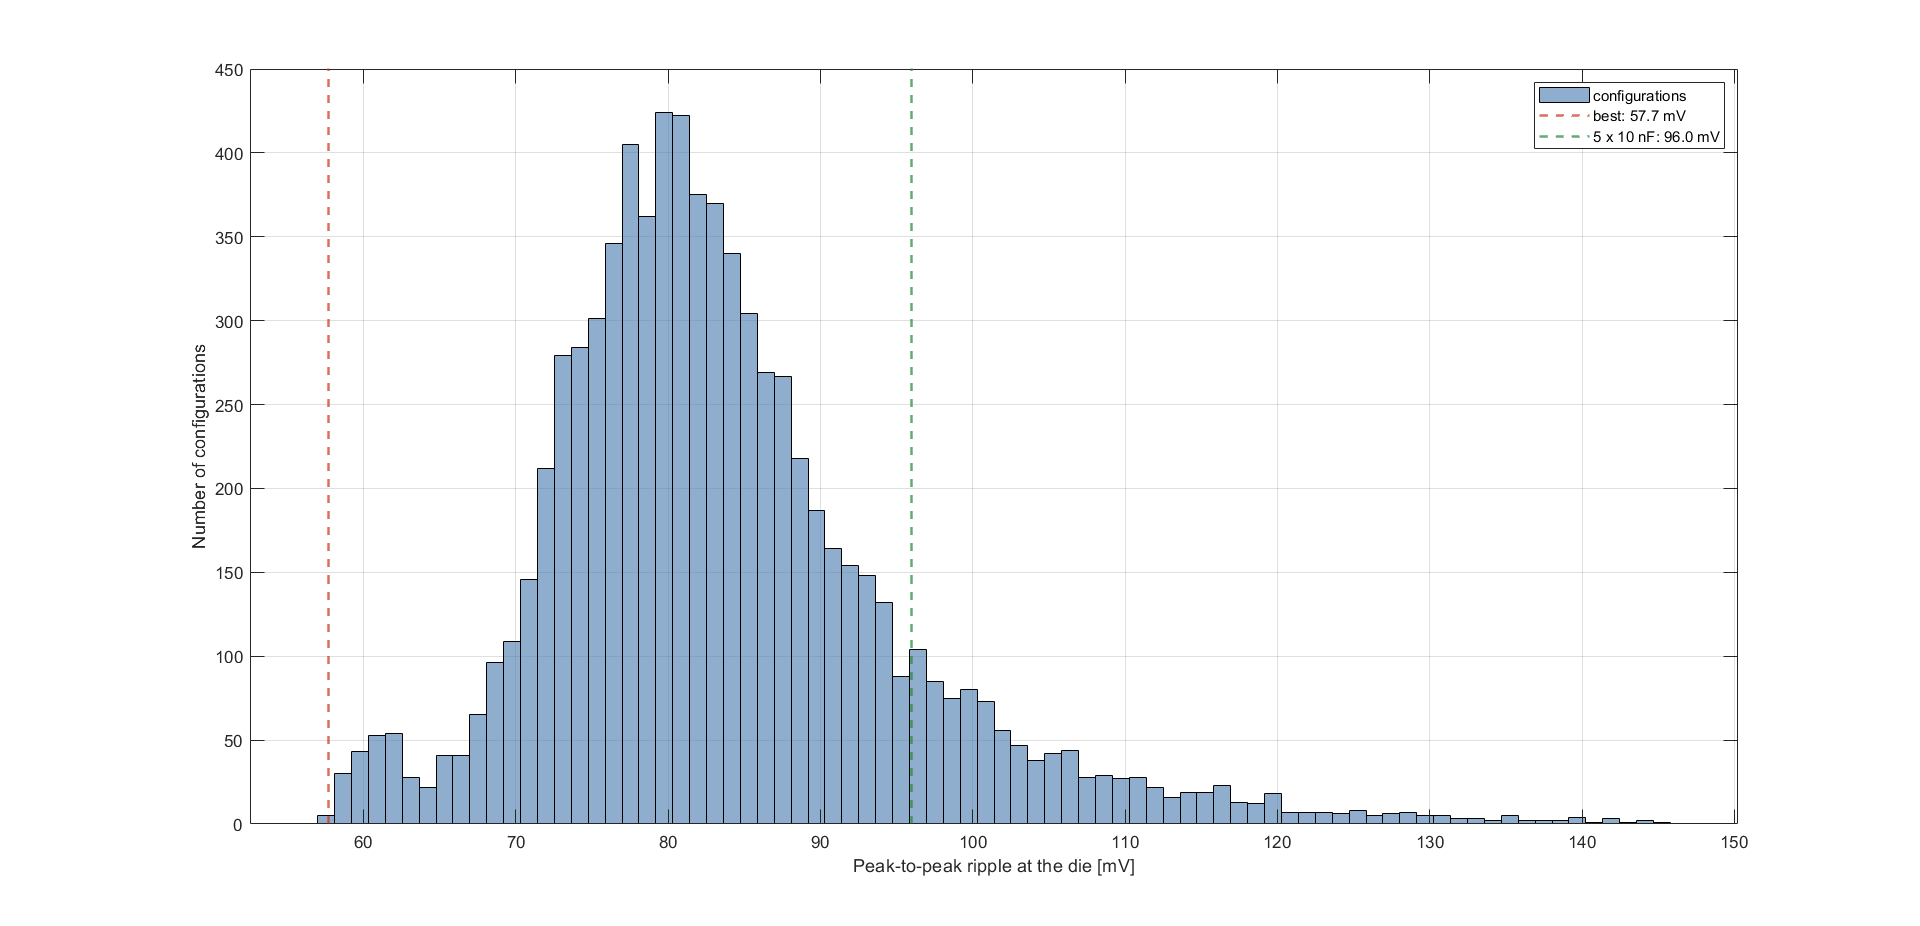
\includegraphics[width=0.8\textwidth]{./eser5/ripple_hist.png}
\caption{Distribution of the predicted peak-to-peak ripple over the 7776 configurations. The dashed lines show the optimal configuration and the configuration with five 10~nF capacitors.}
\label{fig:hist}
\end{figure}

\noindent The result also shows that the best configuration is not the one that gives the lowest peak of the impedance. The ripple depends on the impedance \textit{weighted by the
spectrum of the die current}, as in \eqref{eq:vrip}, and the spectrum is dominated by a line at $100~\text{MHz}$ (amplitude of about $56.5~\text{mA}$), with about $69\%$ of
the power between $50$ and $200~\text{MHz}$. The best configuration is the one that makes the impedance small exactly where the current is large: at $100~\text{MHz}$ the
impedance falls from $2.05~\Omega$ to $0.17~\Omega$, so the amplitude of the dominant line of the ripple falls from about $116~\text{mV}$ to about $10~\text{mV}$.

%%%%%%%%%%%%%%%%%%%%%%%%%%%%%%%%%%%%%%%%%%%%%%%%%%%%%%%%%%

\subsection{AC and transient analysis with the optimal decoupling capacitors}
\label{sec:best}

The optimal configuration has been verified with a direct simulation in LTspice, to check the predictions of the method. The netlists \texttt{pdn\_best\_ac.cir} and
\texttt{pdn\_best\_tran.cir} are the same ones of Exercises~2 and 4, with the five capacitors of \autoref{tab:best} added between the capacitor locations and the ground
(Listing~\ref{lst:best}).

\begin{lstlisting}[language=ltspice, caption={Connection of the optimal decoupling capacitors in the netlists \texttt{pdn\_best\_ac.cir} and \texttt{pdn\_best\_tran.cir}.}, label={lst:best}]
.include "../eser1/pdn.cir"
Xc01 c01 0 GCM033R71A332KA03      * 3.3nF
Xc02 c02 0 GCM033R71A222KA03      * 2.2nF
Xc03 c03 0 GCM033R71A152KA03      * 1.5nF
Xc04 c04 0 GCM033R71A152KA03      * 1.5nF
Xc05 c05 0 GCM033R71A222KA03      * 2.2nF
\end{lstlisting}

%\noindent\\ \textbf{Frequency domain.} The impedance seen from the die is shown in \autoref{fig:zdie_best}, together with the one of the PDN without decoupling capacitors.
\subsubsection{Frequency domain analysis of the PDN with optimal decaps configuration}
The impedance seen from the die with the optimal decaps configuration is shown in \autoref{fig:zdie_best}.\\
%together with the one of the PDN without decoupling capacitors.
The maximum of the impedance falls from $3.06~\Omega$ at $95.9~\text{MHz}$ to $0.829~\Omega$ at $74.9~\text{MHz}$ (the \texttt{.meas} of LTspice gives
$-1.63263~\text{dB}$). The resonance peak is therefore reduced by a factor of about $3.7$, and it is moved away from the $100~\text{MHz}$ line of the die current, where the impedance is now only
$0.17~\Omega$. The maximum and the frequency obtained from \eqref{eq:zdie} are the same ones of LTspice, which confirms that the matrix method reproduces the direct simulation.

\begin{figure}[!h]
\centering
% Replace the placeholder below with the LTspice plot (no decaps and optimal decaps on the same axes):
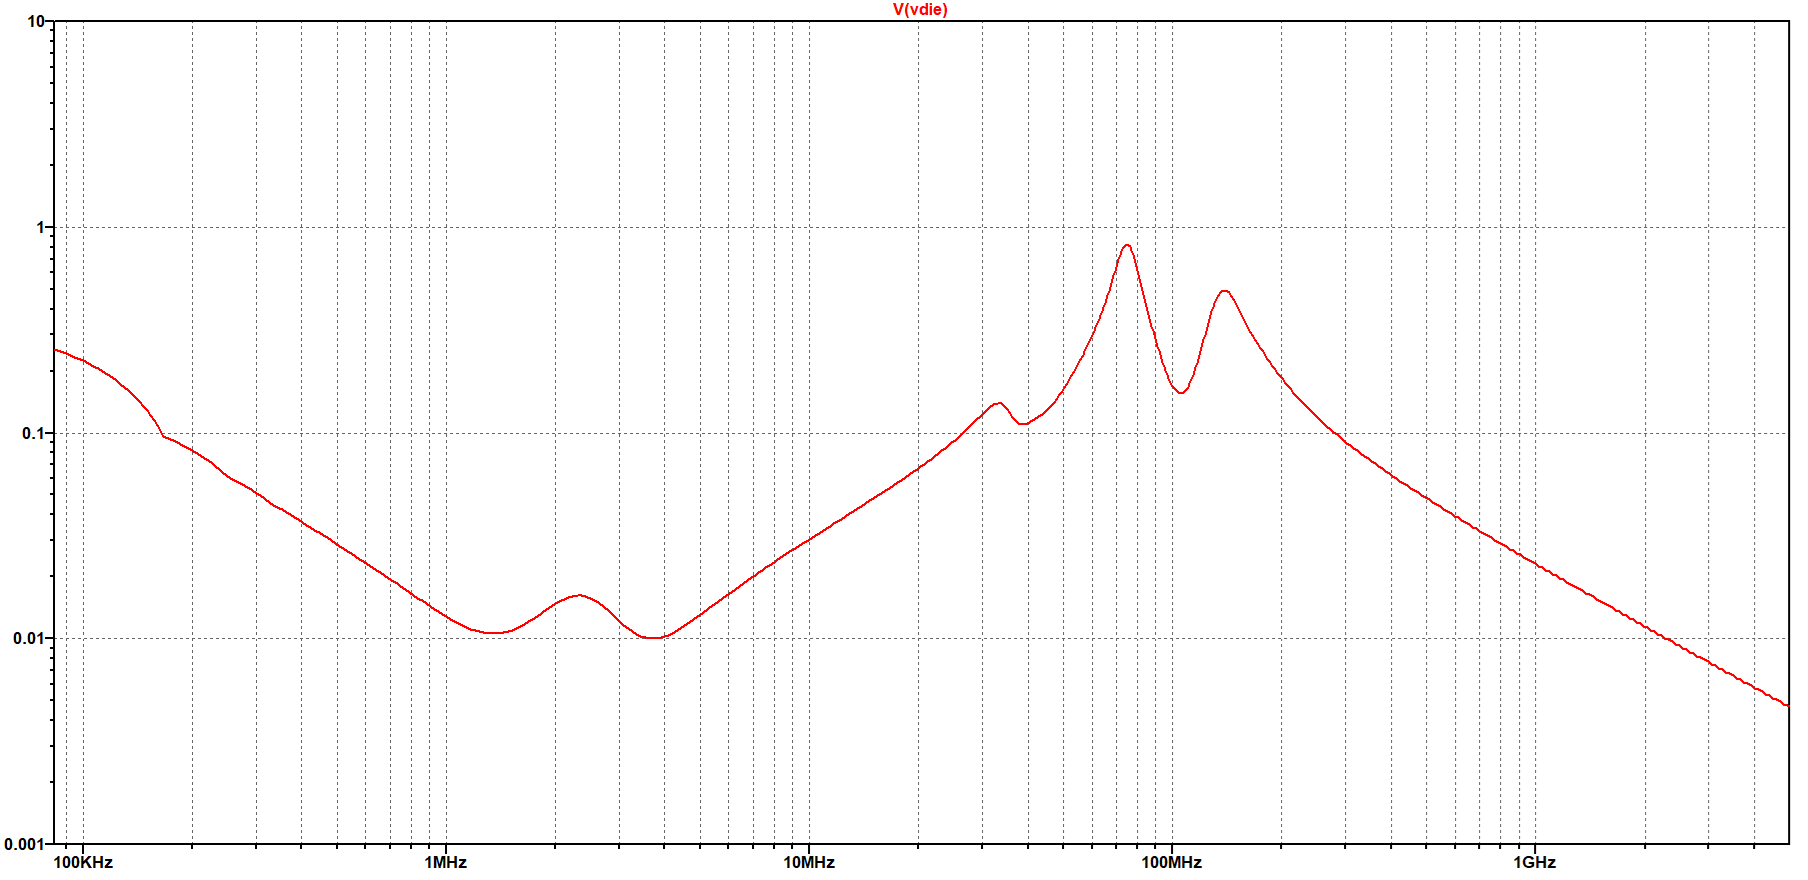
\includegraphics[width=0.95\textwidth]{./eser5/zdie_best.png}
%\fbox{\parbox{0.9\textwidth}{\centering\vspace{3cm} Figure placeholder: $|Z_{die}|$ without decoupling capacitors and with the optimal configuration\vspace{3cm}}}
\caption{Impedance magnitude seen from the die interface with optimal decaps configuration}
\label{fig:zdie_best}
\end{figure}

%\noindent\\ \textbf{Time domain.} The transient simulation uses the same settings of Exercise~4 ($12~\mu\text{s}$, maximum time step of $72~\text{ps}$). The
\subsubsection{Time domain simulation of the PDN with optimal decaps configuration} The transient simulation uses the same settings of Exercise~4 ($12~\mu\text{s}$, maximum time step of $72~\text{ps}$). The
peak-to-peak ripple measured by LTspice over the whole simulation is $59.5~\text{mV}$, against $280.8~\text{mV}$ of the PDN without decoupling capacitors: the ripple is reduced by about $79\%$, that is by a factor of $4.7$.
The waveform is shown in \autoref{fig:vdie_best}.

\begin{figure}[!h]
\centering
% Replace the placeholder below with the LTspice plot of V(vdie) with the optimal decaps:
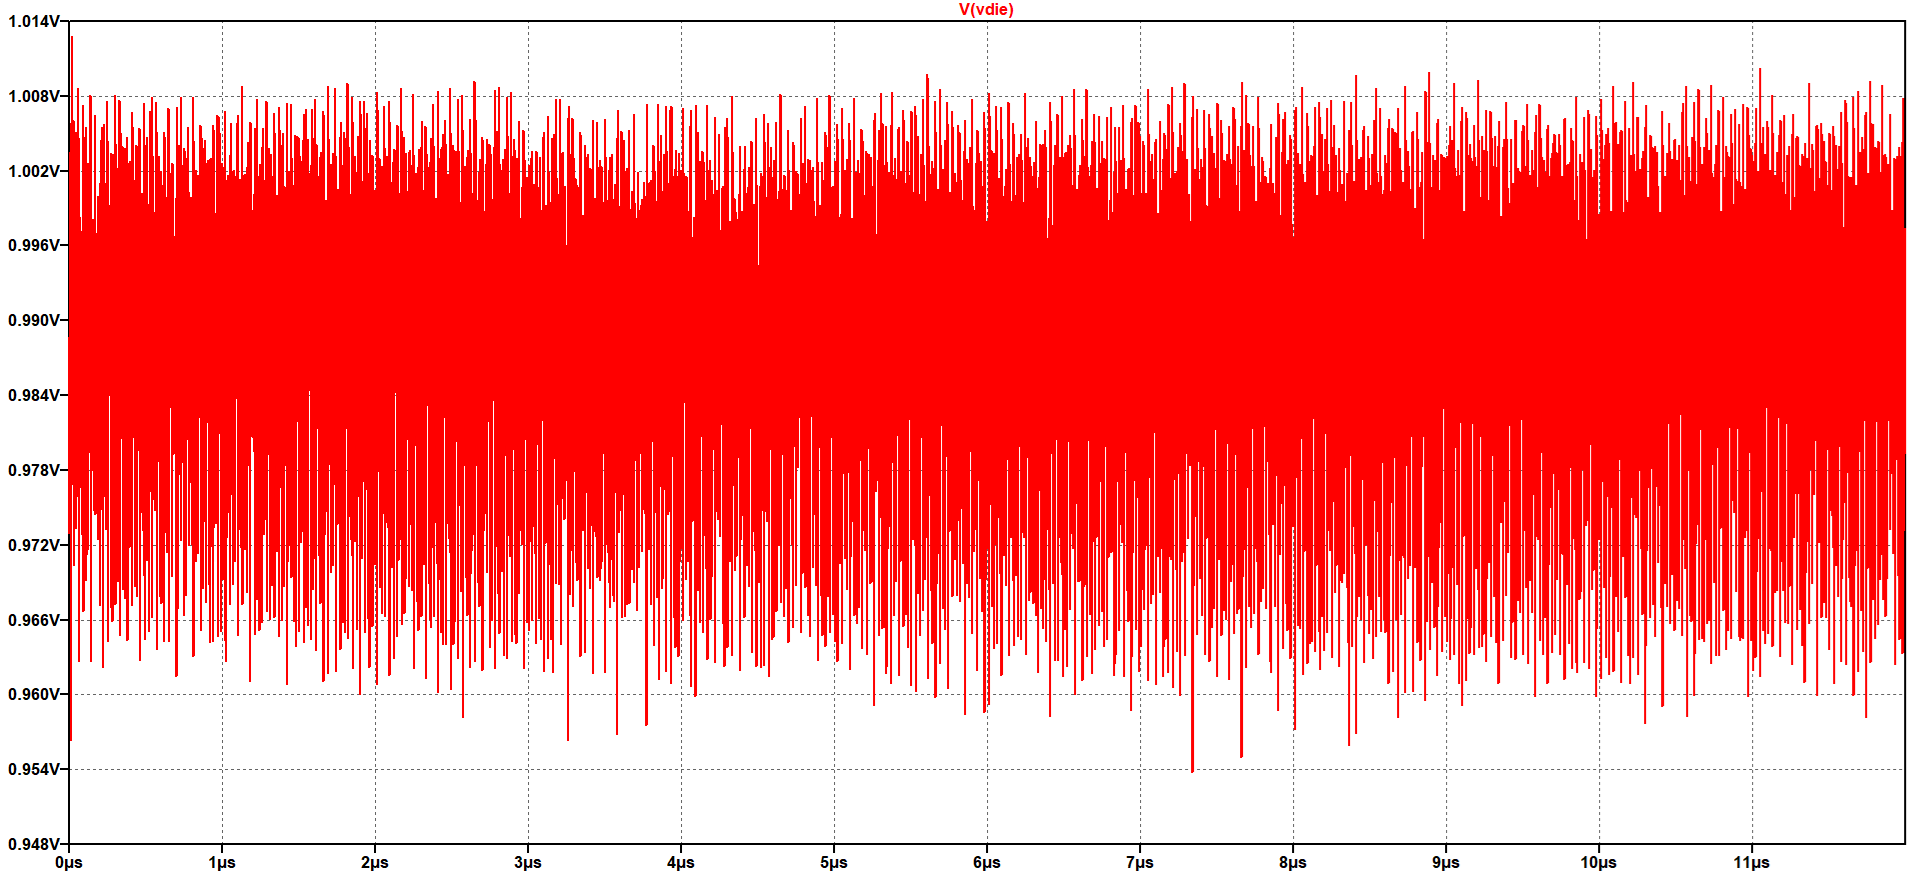
\includegraphics[width=\textwidth]{./eser5/vdie_best.png}
%\fbox{\parbox{0.9\textwidth}{\centering\vspace{3cm} Figure placeholder: $V(\texttt{vdie})$ with the optimal decoupling capacitors\vspace{3cm}}}
\caption{Voltage at the die interface with the optimal decoupling capacitors over the whole simulation ($12~\mu\text{s}$).}
\label{fig:vdie_best}
\end{figure}

\noindent The value predicted by the method, $57.6~\text{mV}$, is slightly lower than the one of the transient. This is expected: the method gives the periodic steady state, while the
transient simulation starts from the DC operating point and includes the start-up of the network, which adds a spike in the first tens of nanoseconds. For the PDN without decoupling capacitors this effect is negligible
($282.2~\text{mV}$ predicted, $280.8~\text{mV}$ simulated), because the ripple is much larger, but it is a few percent of the ripple with the optimal capacitors.
% TODO: if the ripple is measured excluding the start-up (.meas tran vpp_ss PP V(vdie) FROM=0.5u TO=12u), write here the value and say that it is closer to the prediction.

\begin{table}[!h]
\centering
\caption{Comparison between the PDN without decoupling capacitors and with the optimal configuration.}
\label{tab:comp_best}
\begin{tabular}{lcc}
\hline
 & \textbf{No decaps} & \textbf{Optimal decaps} \\
\hline
$\max |Z_{die}|$ [$\Omega$]                          & 3.06 & 0.8286 \\
Frequency of the maximum [MHz]                       & 95.9 & 74.918 \\
$|Z_{die}|$ at 100~MHz [$\Omega$]                    & 2.05 & 0.1702 \\
$V_{pp}$ from the method [mV]                        & 282.2 & 57.6 \\
$V_{pp}$ from the transient (LTspice) [mV]           & 280.8 & 59.5 \\
\hline
\end{tabular}
\end{table}

%%%%%%%%%%%%%%%%%%%%%%%%%%%%%%%%%%%%%%%%%%%%%%%%%%%%%%%%%%%

\subsection{Comparison with other configurations}

To evaluate the benefit of the optimisation, the optimal configuration is finally compared with the PDN without decoupling capacitors and with the six configurations that
use the same capacitor on all the five locations. \autoref{tab:comp_all} collects the impedance and the ripple: the values from the method of \autoref{sec:theory} are
reported together with the ones of the direct LTspice transient simulation.

\begin{table}[!h]
\centering
\caption{Comparison of the configurations. The ripple of the transient simulation is the \texttt{.meas} of LTspice over the whole simulation.}
\label{tab:comp_all}
\begin{tabular}{lcccc}
\hline
\textbf{Configuration} & $\max|Z_{die}|$ [$\Omega$] & $|Z_{die}|_{100~\text{MHz}}$ [$\Omega$] & $V_{pp}$ method [mV] & $V_{pp}$ LTspice [mV] \\
\hline
No decaps             & 3.06 (95.9~MHz)  & 2.05  & 282.2 & 280.8 \\
$5\times$ 10~nF       & 1.86 (120.4~MHz) & 0.443 & 96.5  & --  \\
$5\times$ 6.8~nF      & 1.59 (122.7~MHz) & 0.368 & 83.4  & --  \\
$5\times$ 4.7~nF      & 1.27 (125.3~MHz) & 0.298 & 74.0  & --  \\
$5\times$ 3.3~nF      & 0.894 (131.6~MHz)& 0.173 & 64.0  & --  \\
$5\times$ 2.2~nF      & 0.837 (75.3~MHz) & 0.176 & 60.1  & --  \\
$5\times$ 1.5~nF      & 1.23 (81.1~MHz)  & 0.336 & 86.7  & --  \\
Optimal               & 0.829 (74.9~MHz) & 0.170 & 57.6  & 59.5 \\
\hline
\end{tabular}
\end{table}
% TODO: fill the last column with the .meas results of the six LTspice transient simulations with the same capacitor on the five locations.
% TODO: comment the final table after the simulations: the values of the method are already in the table, they should be confirmed by LTspice.

\noindent With the same capacitor on all the locations, the ripple does not decrease with the capacitance: the five 10~nF capacitors, the largest ones, give the highest ripple among the
configurations with decoupling capacitors, $96.5~\text{mV}$, while the lowest ripple of this group is obtained with $5\times 2.2~\text{nF}$, $60.1~\text{mV}$. In all cases the capacitors reduce the ripple with respect to the
PDN alone by a factor of about three or more. The optimal configuration, which mixes capacitors with different self-resonance frequencies, gives the lowest ripple of all, but its advantage over the best uniform
configuration is small, about $4\%$: the improvement of the optimisation comes mainly from the choice of the right values, and only marginally from their distribution among the five locations.


%\noindent\\ However, all the measurements described above are taken inside the whole simulation window, so they include the initial transient,
%when the voltage is still settling from 0~V to its steady-state value. In order to have a more realistic evaluation of the ripple,
%the first 0.5~$\mu$s of simulation should be excluded, so only the last 11.5~$\mu$s are really significant for the ripple evaluation.
%In this way, all measurements are performed when the voltage has already settled to its steady-state behaviour.\\ As a consequence, a less pessimistic
%scenario is obtained (see last column of \autoref{tab:ripple}), but the measured ripple is still critical, equal to  peak-to-peak, which is  of the supply voltage, and the voltage still goes below 0.95~V and above 1.05~V.